\documentclass[twoside,11pt]{article}
\usepackage[left=1in, right=1in, top=1in, bottom=1in]{geometry}
\usepackage{amsmath}
\usepackage{amssymb}
\usepackage{amsfonts}
\usepackage{mathtools}
\usepackage{amsthm}
\usepackage{thmtools}
\usepackage{fancyhdr}
\usepackage{enumitem}
\usepackage{siunitx}
\usepackage{booktabs}
\usepackage[hidelinks]{hyperref}
\usepackage{sectsty}
\usepackage{mathrsfs} % mathscr
\usepackage{tikz}
\usepackage{pgfplots}
\usepackage{multicol}
\usepackage{listings}
% \usepackage{amsart}
\usepackage{fontspec}
\usepackage{soul}


% allow H option of figure
\usepackage{float}

% math font (libertine)
\usepackage{libertinus-otf}

% braket
\usepackage{braket}

% Chinese support
\usepackage{xeCJK}

% theorem colored box
\usepackage[many]{tcolorbox}

%% equation numbering
\numberwithin{equation}{section} % numbering equations by section
\renewcommand{\theequation}{\arabic{equation}} % remove section number

% tikz library
\usetikzlibrary{
    external,
    decorations,
    calc,
    3d,
}
\tikzexternalize[prefix=tikzpictures/]
\tikzexternaldisable

% physics
% \usepackage{physics}

% define latin modern font environment
\newcommand{\lms}{\fontfamily{lmss}\selectfont} % Latin Modern Roman
% \newcommand{\lmss}{\fontfamily{lmss}\selectfont} % Latin Modern Sans
% \newcommand{\lmss}{\fontfamily{lmtt}\selectfont} % Latin Modern Mono

% % change mathcal shape
% \usepackage[mathcal]{eucal}


% define math operators
\newcommand{\FF}{\mathbb{F}}
\newcommand{\RR}{\mathbb{R}}
\newcommand{\NN}{\mathbb{N}}
\newcommand{\ZZ}{\mathbb{Z}}
\newcommand{\QQ}{\mathbb{Q}}
\newcommand{\XX}{\mathbb{Y}}
\newcommand{\CL}{\mathcal{L}}
% \renewcommand{\d}{\mathrm{d}}
\renewcommand*\d{\mathop{}\!\mathrm{d}}
\DeclareMathOperator*{\argmax}{arg\,max}
\DeclareMathOperator*{\argmin}{arg\,min}
\DeclareMathOperator{\im}{im}
\DeclareMathOperator{\id}{id}
\DeclareMathOperator{\erf}{erf}
\renewcommand{\mod}[1]{\ (\mathrm{mod}\ #1)}

% section font style
\sectionfont{\lms\Large}
\subsectionfont{\lms\normalsize}
\subsubsectionfont{\bf}

% line spreading and break
\hyphenpenalty=5000
\tolerance=20
\setlength{\parindent}{0em}
\setlength\parskip{0.5em}
\allowdisplaybreaks
\linespread{0.9}

% enumerate settings
% no break before enumerate
\setlist[enumerate]{itemsep=2pt,topsep=2pt}
\setlist[itemize]{itemsep=2pt,topsep=2pt}

%%% theorem
%% amsthm theorem
% definition style
\theoremstyle{definition}
\newtheorem{theorem}{\lms Theorem}[section]
\newtheorem{axiom}{\lms Axiom}[section]
\newtheorem{definition}{\lms Definition}[section]
\newtheorem{example}{\lms Example}[section]
\newtheorem{question}{\lms Question}[section]
\newtheorem{exercise}{\lms Exercise}[section]
\newtheorem*{exercise*}{\lms Exercise}
\newtheorem{lemma}{\lms Lemma}[section]
\newtheorem{proposition}{\lms Proposition}[section]
\newtheorem{corollary}{\lms Corollary}[section]
\newtheorem*{theorem*}{\lms Theorem}
\newtheorem{problem}{\lms Problem}
% remark style
\theoremstyle{remark}
\newtheorem*{remark}{\lms Remark}
\newtheorem*{solution}{\lms Solution}
\newtheorem*{claim}{\lms Claim}

%% coloring theorem
% define colors
\colorlet{theoremcolor}{blue!4!white}
\colorlet{examplecolor}{red!3!white}
\colorlet{definitioncolor}{green!3!white}
% theorem
\tcolorboxenvironment{theorem}{
  colback=theoremcolor,
  boxrule=0pt,
  boxsep=1pt,
  left=0pt,right=0pt,top=2pt,bottom=2pt,
  oversize=2pt,
  sharp corners,
  before skip=\topsep,
  after skip=\topsep,
  breakable,
}
% example
\tcolorboxenvironment{example}{
  colback=examplecolor,
  boxrule=0pt,
  boxsep=1pt,
  left=0pt,right=0pt,top=2pt,bottom=2pt,
  oversize=2pt,
  sharp corners,
  before skip=\topsep,
  after skip=\topsep,
  breakable,
}
% definition
\tcolorboxenvironment{definition}{
  colback=definitioncolor,
  boxrule=0pt,
  boxsep=1pt,
  left=0pt,right=0pt,top=2pt,bottom=2pt,
  oversize=2pt,
  sharp corners,
  before skip=\topsep,
  after skip=\topsep,
  breakable,
}


% paragraph indent
\setlength{\parindent}{0em}
\setlength\parskip{0.5em}

\newcommand\Code{PHY3110 SP23}
\newcommand\Ass{Notes}
\newcommand\name{Haoran Sun}
\newcommand\mail{haoransun@link.cuhk.edu.cn}

\title{{\lms \Code \ \Ass}}
\author{\lms \name \ (\href{mailto:\mail}{\mail})}
\date{\lms \today}

\makeatletter
% \let\Title\@title
\let\theauthor\@author
\let\thedate\@date

\fancypagestyle{plain}{%
    \fancyhf{}
    \lhead{\lms\Ass}
    \rhead{\lms\name}
    \rfoot{\lms\thepage}

    % # 页脚自定义
    \fancyfoot[L]{
        \begin{minipage}[c]{0.06\textwidth}
            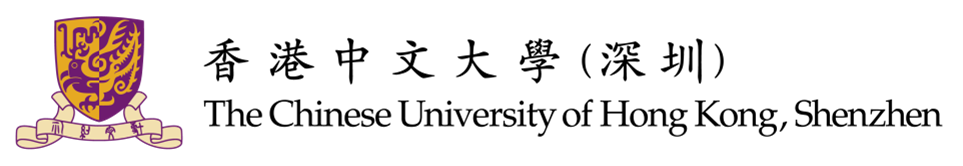
\includegraphics[height=7.5mm]{logo2.png}
        \end{minipage}
    }
}
\fancypagestyle{title}{%
    \fancyhf{}
    \renewcommand{\headrulewidth}{0pt}
    % \lhead{\Title}
    % \rhead{\theauthor}
    \rfoot{\lms\thepage}

    % # 页脚自定义
    \fancyfoot[L]{
        \begin{minipage}[c]{0.06\textwidth}
            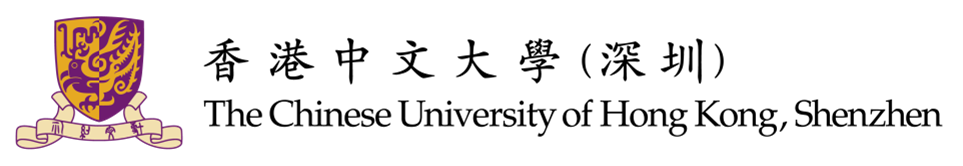
\includegraphics[height=7.5mm]{logo2.png}
        \end{minipage}
    }
}
\fancyfootoffset[L]{0.3cm}

% re-define title format
\makeatletter
\renewcommand{\maketitle}{\bgroup\setlength{\parindent}{0pt}
\begin{flushleft}
  \textbf{\Large\@title}

  \@author
\end{flushleft}\egroup
}
\makeatother

\pagestyle{plain}

% lstlisting settings
\lstset{
    basicstyle=\linespread{0.7}\footnotesize,
    breaklines=true,
    basewidth=0.5em
}


\begin{document}
\maketitle
\thispagestyle{title}
% \begin{multicols*}{2}

% \begin{remark}
%     $V_\epsilon(x)$ is used to denote a $\epsilon$-neighborhood
%     \begin{align*}
%         V_\epsilon(x) = B_\epsilon(x)\setminus\{x\}
%     \end{align*}
% \end{remark}

% \tableofcontents

\setcounter{section}{-1}
\section{Introduction}
\textbf{Grading:} 30\% homework, 30\% midterm, 40\% final.

\textbf{Textbooks:}
\begin{itemize}
    \item H. Goldstein, C. Poole, J. Safko, Classical Mechanics,
    3rd Edition, Pearson.
    \item J.R. Taylor, Classical Mechanics, University Science Books.
    \item T.W.B. Kibble, F.H. Berkshire, Classical Mechanics, 5th Edition,
    Imperial College Press.
    \item 梁昆淼,力学(下册)理论力学,4th Edition,高等教育出版社.
\end{itemize}

Classical mechanics describe the motion of macroscopic objects, which are
not extremely massive and not extremely fast.

\section{Newtonian Mechanics}
Vectorial quantities of motion: position $\mathbf{r}$, 
velocity $\mathbf{v}$, force $\mathbf{F}$,
momentum $\mathbf{p}=m\mathbf{v}$,
angular momentum $\mathbf{L}=\mathbf{r}\times\mathbf{p}$.
Equations of motion are derived from those vector quantities.

Analytical mechanics uses scalar quantities of motion
\begin{itemize}
    \item Kinetic energy $T = \frac{1}{2}m\mathbf{v}^2$
    \item Potential energy $V = V(\mathbf{r})$
\end{itemize}
Equations of motion are derived from those scalar quantities.
\subsection{Newton's Laws}
\begin{theorem}[Newton's 2\textsuperscript{nd} law]
\begin{align}
    \mathbf{F} = \frac{\d \mathbf{p}}{\d t} = m\mathbf{a}
\end{align}
The formula is valid in an inertial frame.
\end{theorem}
Angular momentum $\mathbf{L}$ and torque $\mathbf{N}$ are also related
\begin{align}
    \frac{\d\mathbf{L}}{\d t} &= 
    \frac{\d}{\d t}(\mathbf{r}\times\mathbf{p})
    = \mathbf{r}\times\mathbf{F}
    = \mathbf{N}
\end{align}

Work done by external forces
\begin{align}
    W_{12} &= \int_1^2\mathbf{F}\d\mathbf{s}
    = \int_1^2 m\frac{\d\mathbf{v}}{\d t}\d\mathbf{s}
    = \int_1^2 m\mathbf{v}\d\mathbf{v}
    = \left.\frac{1}{2}m\mathbf{v}^2\right|_1^2
\end{align}

Define a scalar function $V(\mathbf{r})$,
then $\mathbf{F}=-\nabla V(\mathbf{r})$ is a conservative force.
\begin{align}
    \oint \mathbf{F}\d\mathbf{s} = 0
\end{align}

Center of mass of the system
\begin{align}
    \mathbf{R} &= 
    \frac{\sum_i m_i\mathbf{r}_i}{\sum_i m_i}
    =
    \frac{\sum_i m_i\mathbf{r}_i}{M}
\end{align}
Total momentum
\begin{align}
    \mathbf{P} 
    &= 
    \sum_i m_i\mathbf{p}_i
    = M\dot{\mathbf{R}}
\end{align}
Hence $\mathbf{P}$ is conserved if external force $\mathbf{F}^{(e)}$ is
zero.

Total angular momentum
\begin{align*}
    \frac{\d \mathbf{L}}{\d t} &= 
    \frac{\d }{\d t} \sum_i\mathbf{r}_i\times\mathbf{p}_i
    = \sum_i \mathbf{r}_i\times \left(
        \mathbf{F}_i^{(e)} + \sum_j \mathbf{F}_{ij}
    \right)
    = \sum_i\mathbf{r}_i\times\mathbf{F}_i^{(e)}
    + \sum_{ij}\mathbf{r}_i\times\mathbf{F}_{ij}
\end{align*}
Since $\mathbf{r}_{ij}$ parallel to $\mathbf{F}_ij$, then
\begin{align}
    \sum_{ij}\mathbf{r}_i\mathbf{F}_{ij} = 
    \frac{1}{2}\sum_{ij}\mathbf{r}_{ij}\times\mathbf{F}_{ji} = 0
\end{align}
Therefore
\begin{align}
    \frac{\d\mathbf{L}}{\d t} &= \mathbf{N}^{(e)}
\end{align}

Decomposition of the angular momentum
\begin{align}
    \mathbf{L} 
    &= \sum_i\mathbf{r}_i\times\mathbf{p}_i
    = \sum_i(\mathbf{R} + \mathbf{r}_i)\times m_i(\mathbf{V} + \mathbf{v}_i')
    = \sum_i \mathbf{R}\times m_i\mathbf{V}
    + \sum_i\mathbf{r}_i'\times m_i\mathbf{v}_i'
\end{align}

\subsection{Constraints}
Holonomic constraint
\begin{align}
    f(\mathbf{r}_1, \mathbf{r}_2, \dots, \mathbf{r}_N, t) &= 0
\end{align}
Example: rigid body
\begin{align}
    (\mathbf{r}_i-\mathbf{r}_j)^2 - c_{ij}^2 &= 0
\end{align}
Example: non-sliding cylinder
\begin{align*}
    \dot{x} - R\dot{\theta} = 0
    \Rightarrow x - R\theta = \text{const}
\end{align*}
A constraint of the form
\begin{align}
    \sum_i g_i(\mathbf{x}_1,\mathbf{x}_2,\dots,\mathbf{x}_n)\d\mathbf{x}_i = 0
    \Rightarrow
    \d G(\mathbf{x}_1,\dots) = 0
    \Rightarrow
    G(\mathbf{x}_1,\dots) = \text{const}
\end{align}

Non-holonomic constraint: cannot be written in the form of holonomic
constraint.

\subsection{Generalized coordinates}
Suppose we have a $N$-particle system, 
we will have $3N$ DOFs.
With $k$ constraints, we will have $3N-k$ DOFs.
Define $q_1,\dots,q_{3N-k}$ generalized coordinates,
we have
\begin{align}
    \mathbf{r}_i &= \mathbf{r}_i(q_1,\dots, q_{3N-1}, t)
\end{align}

\section{Lagrange Formalism}
\subsection{D'Alembert's Principle}
Hint from the rigid body: internal forces of constraints do not work.

Virtual displacement: $\delta\mathbf{r}_i$
is consistent with the constraints imposed on the system at
a given time
\begin{align}
    \mathbf{r}_i \rightarrow 
    \mathbf{r}_i + \delta\mathbf{r}_i
\end{align}
\begin{theorem}[D'Alembert's principle]
Consider a system in equilibrium
\begin{align}
    \mathbf{F}_i = 0
    \Rightarrow
    \sum_i\mathbf{F}_i\cdot\delta\mathbf{r}_i = 0
\end{align}
Separate $\mathbf{F}_i = \mathbf{F}_i^{(a)} + \mathbf{f}_i$
where $\mathbf{f}_i$ is the constraint force.
Hence
\begin{align}
    \sum_i(\mathbf{F}_i^{(a)} + \mathbf{f}_i)
    \cdot\delta\mathbf{r}_i = 0
    \Rightarrow
    \sum_i\mathbf{F}_i^{(a)}\cdot\delta\mathbf{r}_i = 0
\end{align}
For a system moving under external forces
\begin{align}
    \mathbf{F}_i - \dot{\mathbf{p}}_i = 0
    \Rightarrow
    \sum_i(\mathbf{F}_i - \dot{\mathbf{p}}_i)\delta\mathbf{r}_i = 0
    \Rightarrow
    \sum_i(\mathbf{F}_i^{(a)} - \dot{\mathbf{p}}_i)\delta\mathbf{r}_i = 0
\end{align}
For holonomic constraints
\begin{align}
    \mathbf{r}_i = \mathbf{r}_i(q_1,\dots,q_n,t),\quad
    \mathbf{v}_i = \frac{\d\mathbf{r}_i}{\d t}
    = \frac{\partial \mathbf{r}_i}{\partial t}
    + \sum_j\frac{\partial\mathbf{r}_i}{\partial q_j}\dot{q}_j,\quad
    \delta\mathbf{r}_i = \sum_j\frac{\partial\mathbf{r}_i}{\partial q_j}
    \delta q_j
\end{align}
\end{theorem}
Define generalized force $Q_j$
\begin{align}
    \sum_i\mathbf{F}_i\delta\mathbf{r}_i
    &= \sum_{ij}\mathbf{F}_i\frac{\partial\mathbf{r}_i}{\partial q_j}\delta q_j
    = \sum_j Q_j\delta q_j
\end{align}
Then
\begin{align}
    \sum_i\dot{\mathbf{p}}_i\cdot\delta\mathbf{r}_i
    &= \sum_{ij}m_i\ddot{\mathbf{r}}_i
    \cdot\frac{\partial \mathbf{r}_i}{\partial q_j}\delta q_j
    = 
    \sum_{ij}\left[
        \frac{\d}{\d t}
        \left(m_i\dot{\mathbf{r}}_i\cdot\frac{\partial\mathbf{r}_i}{\partial q_j}\right)
        - m_i\dot{\mathbf{r}}_i\frac{\d}{\d t}\frac{\partial\mathbf{r}_i}{\partial q_j}
    \right]\delta q_j\\
    &= 
    \sum_i\left[
        \frac{\d }{\d t}\left(\frac{\partial T}{\partial\dot{q}_j}\right)
        - \frac{\partial T}{\partial q_j}
    \right]\delta q_j
    = \sum_j Q_j\delta q_j\\
\end{align}
Hence $\forall j$ we have
\begin{align}
    \frac{\d }{\d t}\left(\frac{\partial T}{\partial\dot{q}_j}\right)
    - \frac{\partial T}{\partial q_j}
    - Q_j = 0
    \label{lag0}
\end{align}
Let the potential energy $V=V(\mathbf{r}_i,\dots)=V(q_j,\dots)$,
then we have
\begin{align}
    Q_j &= \sum_i\mathbf{F}_i\frac{\partial\mathbf{r}_i}{\partial q_j}
    = \sum_i -\nabla_i V\frac{\partial\mathbf{r}_i}{\partial q_j}
    = -\frac{\partial V}{\partial q_j}
\end{align}
Therefore
\begin{align}
    \frac{\d }{\d t}\left(\frac{\partial (T-V)}{\partial\dot{q}_j}\right)
    - \frac{\partial (T-V)}{\partial q_j}
    - Q_j = 0
\end{align}
\begin{theorem}[Langrange's equation]
Define $L=T-V$, then
\begin{align}
    \frac{\d }{\d t}\left(\frac{\partial L}{\partial\dot{q}_j}\right)
    - \frac{\partial L}{\partial q_j}
    = 0
\end{align}
The choice of Lagrangian is not unique, $L'$ where
\begin{align}
    L' = L + \frac{\d F(q, t)}{\d t}
\end{align}
will give the same equations of motion as $L$.
\end{theorem}

\begin{example}[Lagrange's formalism]\
\begin{enumerate}[label=\arabic*)]
\item For a single particle moving under force $\mathbf{F}$
\begin{align*}
    L(\mathbf{x}, \dot{\mathbf{x}}, t) &= \frac{1}{2}m\dot{\mathbf{x}}^2 + \mathbf{F}\cdot\mathbf{x}
\end{align*}

\item Motion in a 2D plane using polar coordinates
\begin{align*}
    L(r, \theta, \dot{r}, \dot{\theta}, t) &= 
    \frac{1}{2}m(\dot{r}^2 + r^2\dot{\theta}^2)
    + F\cdot\mathbf{r}
\end{align*}
Generalized forces
\begin{align*}
    Q_r &= \mathbf{F}\cdot\frac{\partial\mathbf{r}}{\partial r}
    = \mathbf{F}\cdot\mathbf{e}_r\\
    Q_\theta &= \mathbf{F}\cdot\frac{\partial\mathbf{r}}{\partial\theta}
    = \mathbf{F}\cdot r\mathbf{e}_\theta
\end{align*}
where
\begin{align*}
    \mathbf{e}_r &= \begin{bmatrix}
        \cos\theta\\ \sin\theta
    \end{bmatrix}\quad
    \mathbf{e}_\theta = \begin{bmatrix}
        -\sin\theta\\ \cos\theta
    \end{bmatrix}
\end{align*}
Equations of motion
\begin{align*}
    m\ddot{r} - mr\dot{\theta}^2 &= \mathbf{F}\cdot\mathbf{e}_r\\
    mr^2\ddot{\theta} + 2mr\dot{r}\dot{\theta} &= r\mathbf{F}_\theta
\end{align*}

\item Atwood's machine
\begin{align*}
    L &= \frac{1}{2}(M_1+M_2)\dot{x}^2 + 
    M_1g x + M_2 g(l-x)
\end{align*}
The equation of motion is
\begin{align*}
    \frac{\d}{\d t}\frac{\partial L}{\partial \dot{x}}
    - \frac{\partial L}{\partial x} &= 0\\
    \Rightarrow (M_1 + M_2)\ddot{x} &= (M_1 - M_2)g
\end{align*}

\end{enumerate}
\end{example}

Suppose we have a potential dependent on velocity (generalized potential)
and the generalized force is defined as
\begin{align}
    U &= U(q_j,\dot{q}_j), \quad
    Q_j = -\frac{\partial U}{\partial q_j} 
    + \frac{\d }{\d t}\frac{\partial U}{\partial\dot{q}_j}
\end{align}
Define $L = T-U$, then we still have
\begin{align}
    \frac{\d }{\d t}\frac{\partial L}{\partial \dot{q}_j} - \frac{\partial L}{\partial q_j} &= 0
\end{align}
\begin{example}[Lorentz force on a moving charge]
The Lorentz force
\begin{align*}
    \mathbf{F} &= 
    q(\mathbf{E} + \mathbf{v}\times\mathbf{B})
\end{align*}
Define the scalar and vector potentials
\begin{align*}
    E &= -\nabla\phi - \frac{\partial \mathbf{A}}{\partial t},\quad
    \mathbf{B} = \nabla\times\mathbf{A}
\end{align*}
Hence
\begin{align*}
    \mathbf{F} &= 
    q\left[
        -\nabla\phi - \frac{\partial \mathbf{A}}{\partial t}
        + \mathbf{v}\times(\nabla\times\mathbf{A})
    \right]
\end{align*}

\end{example}

\subsection{Hamilton's principle, variational principle}
Configuration space: a space formed by the set of generalized coordinates.
\begin{align}
    (q_1, q_2, \dots, q_n)\text{ as function of $t$}
\end{align}
\begin{theorem}[Hamilton's principle]
Define the action integral $I$, where $L=T-V$ or $L=T-U$ ($U$ is the generalized
potential)
\begin{align}
    I =  \int_{t_1}^{t_2}L\d t
\end{align}
Then the variation of the action integral equals to zero
\begin{align}
    \delta I &= 
    \delta \int_{t_1}^{t_2}L(q_1,\dots, q_n,\dot{q}_1,\dots,\dot{q}_n)\d t
    = 0
\end{align}
Add small variation on the path
\begin{align}
    q_i(t, \alpha) &= q_i(t) + \alpha\eta(t)
\end{align}
where $\eta(t_1)=\eta(t_2)=0$.
Then the action will be the function of $\alpha$, $I=I(\alpha)$.
Hence
\begin{align}
    \delta I &= 
    \int_{t_1}^{t_2}\left(\sum_i \frac{\partial L}{\partial q_i}\delta q_i
    + \frac{\partial L}{\partial \dot{q}_i}\delta\dot{q}_i\right)\d t
\end{align}
Change the order of differentiation $\delta\dot{q}_i = \d \delta q_i/\d t$, then
\begin{align}
    \delta I(\alpha) &= 
    \int_{t_1}^{t_2}\sum_i\left[
        \frac{\partial L}{\partial q_i}\delta q_i
        - \frac{\d}{\d t}\left(\frac{\partial L}{\partial\dot{q}_i}\right)\delta q_i
        \right]\d t
        + \sum_i\frac{\partial L}{\partial\dot{q}_i}\delta q\large|_{t_1}^{t_2}\\
    &= 
    \int_{t_1}^{t_2}\sum_i\left[
        \frac{\partial L}{\partial q_i}
        - \frac{\d}{\d t}\left(\frac{\partial L}{\partial\dot{q}_i}\right)
    \right]\delta q_i\d t = 0 \\
    \Rightarrow
    & \frac{\d}{\d t}\left(\frac{\partial L}{\partial\dot{q}}\right)
    - \frac{\partial L}{\partial q_i} = 0
\end{align}
\end{theorem}

\begin{example}[Shortest path problem]
$y=y(x)$, $\d s = \sqrt{\d x^2 + \d y^2}$, then the action integral (path) is
\begin{align}
    I &= \int_1^2\d s = 
    \int_1^2\sqrt{1+\dot{y}^2}\d x
\end{align}
Apply the Lagrange's equation we get
\begin{align}
    \frac{\d }{\d x}\frac{\d \sqrt{1+\dot{y}^2}}{\d \dot{y}} = 0
    \Rightarrow \frac{\d\dot{y}}{\d x} = 0
    \Rightarrow y = ax + b
\end{align}
\end{example}

\begin{example}[Solid of revolution]
Differential of area $2\pi x\d s = 2\pi x\sqrt{1+\dot{y}^2}\d x$,
then the total area is
\begin{align}
    \int_1^2 2\pi x\sqrt{1+\dot{y}^2}\d x
\end{align}
Define the Lagrangian $L(x, y, \dot{y}) = 2\pi x\sqrt{1+\dot{y}^2}$,
by Lagrange's equation we can get
\begin{align}
    \frac{x\dot{y}}{\sqrt{1+\dot{y}^2}} = \text{const}
    \Rightarrow y = a\cosh\frac{x}{a} + b
\end{align}
\end{example}

\begin{example}[The curve of fastest descent]
Question: along which trajectory from point 1 to point 2,
the time is shortest?
The total time is
\begin{align}
    T &= \int_1^2
    \frac{\d s}{v}
    = \int_1^2\frac{\d s}{\sqrt{2gy}}
\end{align}
According to Newton's laws we have $y=gv^2$, then
\begin{align}
    T &= \int_1^2\frac{\sqrt{1+\dot{y}^2}}{\sqrt{2gy}}\d x
\end{align}
Then we have $L(x, y, \dot{y})$ and we get \hl{check drivation}
\begin{align}
    \frac{\dot{y}}{2y} + \frac{y\ddot{y}}{1 + \dot{y}^2} &= 0\\
    \Rightarrow \frac{\d}{\d x}\ln[y(1+\dot{y}^2)] &= 0
\end{align}
which means that $y(1+\dot{y}^2)=\text{const}$.
The solution is $x=a(\theta-\sin\theta)$, $y=a(1-\cos\theta)$.
\end{example}

\subsection{Constraint}
Holonomic constraints
\begin{align}
    f(q_1,\dots,q_n,t) &= 0
\end{align}
Non-holonomic constraints
\begin{align}
    f(q_1,\dots,q_n;\dot{q}_1,\dots,\dot{q}_n;t) &= 0
\end{align}
Sometimes we can convert $f(\dot{q}_i)=0$ to $f'(q_i)=0$.
\begin{example}[Rolling cylinder]
Rolling cylinder without sliding has the constraint
\begin{align}
    \dot{x} - R\dot{\theta} = 0
    \Rightarrow x-R\theta = \text{const}
\end{align}
\tikzexternalenable
\begin{figure}[H]
    \centering
    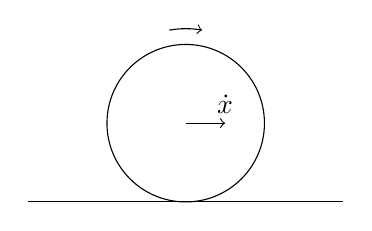
\begin{tikzpicture}
        \draw (-2,0)--(2,0);
        \draw (0,1) circle (1);
        \draw[->] (0,1)+(100:1.2) arc (100:80:1.2);
        \draw[->] (0,1) -- (0.5, 1) node[above] {$\dot x$};
    \end{tikzpicture}
\end{figure}
\tikzexternaldisable
\end{example}

A commonly encountered type of non-holonomic constraint is linear constraint equations
\begin{align}
    \sum_{k=1}^n a_{ik}\frac{\d q_k}{\d t} + a_i t &= 0
\end{align}
For the virtual displacement $\delta q_i$
\begin{align}
    \sum_{k=1}^n a_{ik}\delta q_k &= 0
\end{align}

Suppose $q_i$ are not independent, then the Euler-Lagrange's equation
could not hold.
\begin{align*}
    \int_{t_1}^{t_2}\sum_i\left[
        \frac{\partial L}{\partial q_i}
        - \frac{\d}{\d t}\left(\frac{\partial L}{\partial\dot{q}_i}\right)
    \right]\delta q_i\d t = 0 
    \nRightarrow
    \frac{\d}{\d t}\left(\frac{\partial L}{\partial\dot{q}}\right)
    - \frac{\partial L}{\partial q_i} = 0
\end{align*}
Include the constraint equation of $q_i$ into the equation
\begin{align}
    \sum_{k=1}^n a_{ik}\delta q_k &= 0
    \Rightarrow
    \sum_{i=1}^m \lambda_i\sum_{k=1}^n a_{ik}\delta q_k = 0
\end{align}
Hence
\begin{align*}
    \int_{t_1}^{t_2}\sum_{k=1}^n\left[
        \frac{\partial L}{\partial q_k}
        - \frac{\d}{\d t}\left(\frac{\partial L}{\partial\dot{q}_k}\right)
        + \sum_{i=1}^m\lambda_i a_{ik}
    \right]\delta q_k\d t = 0 
\end{align*}
Let $q_1,\dots,q_{n-m}$ be independent generalized coordinate,
$q_{n-m+1},\dots,q_n$ dependent generalized coordinates (i.e., they can
be expressed by $q_1,\dots,q_{n-m}$).
Choose $\lambda_i$ s.t.
\begin{align}
    \frac{\partial L}{\partial q_k}
    - \frac{\d}{\d t}\left(\frac{\partial L}{\partial\dot{q}_k}\right)
    + \sum_{i=1}^m\lambda_i a_{ik}
    = 0
\end{align}
$\forall k = n-m+1,\dots,n$.
In conclusion, we have $q_1,\dots,q_n,\lambda_1,\dots,\lambda_m$ overall
$n+m$ unknowns, and $n$ Lagrange's equations and $m$ constraint equations
overall $n+m$ equations.
\begin{remark}\ 
\begin{enumerate}[label=\arabic*)]
\item It is inconvenient to reduce all $q_k$s to independent 
coordinates
\item If we are interested in the constraint forces
\begin{align*}
    \sum_{k=1}^n a_{ik}\d q_k + a_{it}\d t = 0
\end{align*}
where 
\begin{align*}
    a_{ik} &= \frac{\partial f_i}{\partial q_k},\quad
    a_{it} = \frac{\partial f_i}{\partial t}
\end{align*}
Then
\begin{align*}
    \d f_i &= \frac{\partial f_i}{\partial q_k}\d q_k + 
    \frac{\partial f_i}{\partial t}\d t
    \Rightarrow \d f_i = 0,~f_i=\text{const}
\end{align*}
\end{enumerate}
\end{remark}

\begin{example}[Hoop rooling down an inclined plane]\
\tikzexternalenable
\begin{figure}[H]
    \centering
    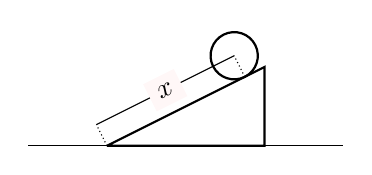
\begin{tikzpicture}
        \draw (0,0)--(4,0);
        \draw[thick] (1,0) -- (3,0) -- (3,1) -- (1,0);
        \draw[thick] (2.75,0.875) arc ({-atan(2)}:{360-atan(2)}:0.3);
        \draw[densely dotted] (2.75,0.875) --++ ({180-atan(2)}:0.3);
        \draw[densely dotted] (1,0) --++ ({180-atan(2)}:0.3);
        \draw ($ (2.75,0.875) + ({180-atan(2)}:0.3) $) -- 
              node[midway,sloped,fill=examplecolor] {$x$}
              ($ (1,0) + ({180-atan(2)}:0.3) $);
    \end{tikzpicture}
\end{figure}
\tikzexternaldisable
The constraint equation writes
\begin{align*}
    \dot{x} - r\dot{\theta} = 0
    \Rightarrow x - r\theta = \text{const}
\end{align*}
$a_x=1$, $a_\theta = -r$, $a_t=0$.

Energy terms are
\begin{align*}
    T &= 
    T_\text{COM} + T_\text{relative}
    = \frac{1}{2}M\dot{x}^2 + \frac{1}{2}M(r\dot{\theta})^2\\
    V &= Mg(l-x)\sin\phi\\
    \Rightarrow
    L &=  \frac{1}{2}M\dot{x}^2 + \frac{1}{2}M(r\dot{\theta})^2
    - Mg(l-x)\sin\phi
\end{align*}
Then we can write the Lagrange's equation with Lagrange's multipliers
\begin{align*}
    \frac{\partial L}{\partial x} - \frac{\d }{\d t}\frac{\partial L}{\partial \dot{x}}
    + a_x\lambda &= 0\\
    \Rightarrow
    Mg\sin\phi - M\ddot{x} + \lambda &= 0\\
    -Mr^2\ddot{\theta} - \lambda r &= 0\\
    \dot{x} &= r\dot{\theta}\Rightarrow
    \ddot{x} = r\ddot{\theta}
\end{align*}
we can get $M\ddot{x} = Mr\ddot{\theta} = -\lambda$ and 
$\ddot{x} = (g\sin\phi)/2$.
Note that $\lambda$ is the constraint force (in this case $\lambda$
is the frictional force).
\hl{check derivation}
\end{example}

\subsection{Lagrangian for Lorentz force}
\begin{definition}[Cylic coordinate]
The generalized coordinate $q_i$ is cyclic (ignorable) if 
\begin{align}
    \frac{\partial L}{\partial q_i} &= 0
\end{align}
It implies the generalized momentum $p_i$ is conserved.
\end{definition}
The Lorentz force is given by
\begin{align}
    \mathbf{F} &= 
    q[\mathbf{E} + \mathbf{v}\times\mathbf{B}]
    \label{eq-EMEOM}
\end{align}
Where
\begin{align}
    \mathbf{E} &= -\nabla\phi - \frac{\partial A}{\partial t},\enskip
    \mathbf{B} = \mathbf{v}\times\mathbf{A}
\end{align}
Hence, by defining the Lagrangian
\begin{align}
    L &= 
    \frac{1}{2}m\mathbf{v}^2 - q\phi + q\mathbf{A}\cdot\mathbf{v}
\end{align}
Applying the Lagrange's equation we can get the EOM (eq. \ref{eq-EMEOM}).

\subsection{Conservation \& symmetry of the system}
\textbf{Rotational symmetry.}
Let $q_j$ be one of the rotational angle of spacial coordinate $\mathbf{r}_i$.
Hence
\begin{align}
    \d\mathbf{r}_i &= 
    \mathbf{n}_j\times\mathbf{r}_i\d q_j
    \Rightarrow
    \frac{\partial\mathbf{r}_i}{\partial q_j} = 
    \mathbf{n}_j\times\mathbf{r}_i\d q_j
\end{align}
where $\mathbf{n}_j$ is the normal vector of the rotation axis of $q_j$.
Hence the generalized force of $q_j$ writes
\begin{align}
    Q_{q_j} &= -\frac{\partial V}{\partial q_j} = 
    -\sum_k\frac{\partial V}{\partial\mathbf{r}_k}\frac{\partial\mathbf{r}_k}{\partial q_j}
    = -\frac{\partial V}{\partial\mathbf{r}_i}\frac{\partial\mathbf{r}_i}{\partial q_j}
    = \mathbf{F}_i\cdot(\mathbf{n}_j\times\mathbf{r}_i)
    = \mathbf{n}_j\cdot(\mathbf{r}_i\times\mathbf{F}_i)
    = \mathbf{n}_j\cdot\mathbf{N}_i
\end{align}
where $\mathbf{N}_i$ stands for the torque on the $i$\textsuperscript{th} particle.
The generalized momentum of $q_j$ writes
\begin{align}
    p_{q_j} &=
    \frac{\partial T}{\partial\dot{q}_j}
    = \sum_k\frac{\partial T}{\partial\dot\mathbf{r}_k}\frac{\partial\mathbf{r}_i}{\partial q_j}
    = \sum_k m_k\dot\mathbf{r}_k\cdot\frac{\partial\dot\mathbf{r}_k}{\partial\dot q_j}
    = m_i\dot\mathbf{r}_i\cdot(\mathbf{n}_j\times\mathbf{r}_i)
    = \mathbf{n}_j\times (\mathbf{r}_i\times m_i\dot\mathbf{r}_i)
    = \mathbf{r}_j\times\mathbf{L}_i
\end{align}
where $\mathbf{L}_i$ stands for the angular momentum of the $i$\textsuperscript{th} particle.
Hence, the rotational invariance implies the conservation of angular momentum.

\textbf{Time translation}
\begin{align}
    \frac{\d}{\d t}L &= 
    \sum_i\frac{\partial L}{\partial q_i}\dot{q}_i
    + \frac{\partial L}{\partial \dot{q}_i}\ddot{q}_i
    + \frac{\partial L}{\partial t}\\
    &= \sum_i\frac{\d}{\d t}\frac{\partial L}{\partial\dot{q}_i}\dot{q}_i
    + \frac{\partial L}{\partial \dot{q}_i}\ddot{q}_i
    + \frac{\partial L}{\partial t}\\
    &= \frac{\d}{\d t}\sum_i\left(\frac{\partial L}{\partial\dot{q}_i}\dot{q}_i\right)
    + \frac{\partial L}{\partial t}\\
    \Rightarrow &
    \frac{\partial L}{\partial t} + 
    \frac{\d}{\d t}\underbrace{\left(
    \sum\frac{\partial L}{\partial\dot{q}_i}q_i - L
    \right)}_{H}
    = 0
\end{align}
Note that
\begin{align}
    \sum_i\frac{\partial L}{\partial\dot{q}_i}\dot{q}_i &= 2T
\end{align}
\begin{proof}
Suppose $r_i$ does not have explicit time dependence
\begin{align*}
    T &= \sum_i \frac{1}{2}m_i\dot{r}_i^2
    = \sum_i \frac{1}{2}m_i\left(
        \sum_j\frac{\partial r_i}{\partial q_j}\dot{q}_j
        + \frac{\partial r_i}{\partial t}
    \right)^2\\
    &= \sum_{ijk}
    \frac{1}{2}m_i\frac{\partial r_i}{\partial q_j}
    \frac{\partial r_i}{\partial q_k}\dot{q}_j\dot{q}_k\\
    \Rightarrow
    \sum_i\frac{\partial L}{\partial\dot{q}_i}\dot{q}_i
    &= \sum_i \dot{q}_i \sum_{jk}
    m_k\frac{\partial r_k}{\partial q_i}\frac{\partial r_k}{\partial q_k}
    \dot{q}_k = 2T\qedhere
\end{align*}
\end{proof}
Hence we can define Hamiltonian $H = T+V$ which stands for the total energy,
and $H$ conserved if $L$ doesn't depend on time explicitly.

\begin{example}[Two blocks]\
Let $M$ be the mass of the big block,
$m$ be the mass of the small block.
Define two generalized coordinates:
$X$ stand for the position of COM of the big block,
$q$ stand for the position of COM of the small block
(sloped). 
\tikzexternalenable
\begin{figure}[H]
    \centering
    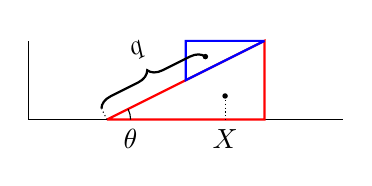
\begin{tikzpicture}
        \draw (0,0)--(4,0);
        \draw (0,0)--(0,1);
        \draw[red,thick] (1,0)--(3,0)--(3,1)--(1,0);    % large block
        \draw[blue,thick] (3,1)--(2,1)--(2,0.5)--(3,1); % small block
        \node[circle,fill,inner sep=0.7pt] at (2.5,0.3) {}; % COM large block
        \node[circle,fill,inner sep=0.7pt] at (2.25,0.8) {}; % COM small block
        \draw[densely dotted] (2.5,0.3)--(2.5,0) node[below,text opacity=1] {$X$}; % X label
        \draw (1,0)+(0:0.3) node[below] {$\theta$} arc (0:atan(1/2):0.3); % theta helper line
        \draw[densely dotted] (1,0)--++ ({180 - atan(2)}:0.15652); % q helper line (left)
        \draw[thick,decorate,decoration={brace,amplitude=5pt}]
            ($ (1,0)+({180-atan(2)}:0.15652) $) -- node[midway,sloped,above=6pt] {$q$} (2.25,0.8); % q brace
    \end{tikzpicture}
\end{figure}
\tikzexternaldisable
Hence we can easily define the Lagrangian
\begin{align*}
    L &= 
    \frac{1}{2}M\dot{X}^2
    + \frac{1}{2}m[
        (\dot{X} + \dot{q}\cos\theta)^2
        + \dot{q}^2\sin^2\theta
    ] - mgq\sin\theta
\end{align*}
There is no $X$ dependence on the system, hence
$X$ is a cyclic coordinate.
\begin{align*}
    \frac{\d}{\d t}\frac{\partial L}{\partial\dot{X}}
    &= \frac{\d}{\d t}M\dot{X} + m(\dot{X} + \dot{q}\cos\theta) = 0\\
    \Rightarrow &M\dot{X} m(\dot{X} +\dot{q}\cos\theta) = p_X = \text{const}
\end{align*}
\end{example}



\section{The Central Force Problem}
\subsection{Reduction to the equivalent one-body problem}
For the two-body problem, we have two choices of
generalized coordinate
\begin{enumerate}[label=(\alph*)]
    \item $\mathbf{r}_1$, $\mathbf{r}_2$ stand for spacial coordinates of two
    masses
    \item $\mathbf{R}$ spacial coordinate of the COM, $\mathbf{r}=\mathbf{r}_1-\mathbf{r}_2$
\end{enumerate}
Hence, we can rewrite the kinetic energy in terms of $\mathbf{R}$ and $\mathbf{r}$
\begin{align}
    T &= \frac{1}{2}m_1\dot\mathbf{r}_1^2 + \frac{1}{2}m_2\dot\mathbf{r}_2^2\\
    &= \frac{1}{2}m_1\left(\dot\mathbf{R}+\frac{m_2}{m_1+m_2}\dot\mathbf{r}\right)^2
    + \frac{1}{2}m_2\left(\dot\mathbf{R}-\frac{m_1}{m_1+m_2}\dot\mathbf{r}\right)^2\\
    &= \frac{1}{2}(m_1+m_2)\dot\mathbf{R}^2 + \frac{m_1m_2}{m_1+m_2}\dot\mathbf{r}^2
    = \frac{1}{2}M\dot\mathbf{R}^2 + \frac{1}{2}\mu\dot\mathbf{r}^2
\end{align}
Hence we can write the Lagrangian
\begin{align}
    L &= 
    \frac{1}{2}M\dot\mathbf{R}^2 + \frac{1}{2}\mu\dot\mathbf{r}^2 - V
\end{align}
Suppose $V=V(\mathbf{r})$, then $\mathbf{R}$ is a cyclic coordinate,
We have $\dot\mathbf{R}=\text{const}$, and we can drop $\dot{\mathbf{R}}$
terms in $L$.
Moreover, if $V=V(\|\mathbf{r}\|)$, the total angular momentum is conserved.

Use $r$, $\theta$ as generalized coordinates, we have
\begin{align}
    L &= \frac{1}{2}\mu(\dot{r}^2 + r^2\dot{\theta}^2) - V(r)
\end{align}
Easy to find that $\theta$ is cyclic, hence
\begin{align}
    \frac{\d}{\d t}\frac{\partial L}{\partial\dot\theta}
    &= \frac{\d}{\d t}\mu r^2\dot\theta = 0
    \Rightarrow p_\theta = \mu r^2\dot{\theta} = L= \text{const}
\end{align}
\begin{theorem}[Kepler's 2\textsuperscript{nd} law]
Radius vector sweeps out equal areas in equal time.
\end{theorem}



% \end{multicols*}
\end{document}

